\documentclass[conference]{IEEEtran}
\IEEEoverridecommandlockouts

\usepackage{cite}
\usepackage{amsmath,amssymb,amsfonts}
\usepackage{algorithmic}
\usepackage{graphicx}
\usepackage{textcomp}
\usepackage{xcolor}
\usepackage{booktabs}
\usepackage{url}
\usepackage{tikz}
\usetikzlibrary{positioning,arrows.meta,calc,fit}
\def\BibTeX{{\rm B\kern-.05em{\sc i\kern-.025em b}\kern-.08em
    T\kern-.1667em\lower.7ex\hbox{E}\kern-.125emX}}
\begin{document}

\title{A From-Scratch CUDA Forward-Pass Inference Engine for a LeNet-Style MNIST CNN}

\author{\IEEEauthorblockN{Ashish Dasu}
\IEEEauthorblockA{\textit{Khoury College of Computer Sciences} \\
\textit{Northeastern University}\\
Boston, MA, USA \\
dasu.a@northeastern.edu}}

\maketitle

\begin{abstract}
I build a forward-pass inference engine for a LeNet-style MNIST
convolutional network in C++ and CUDA, with no deep-learning framework
at runtime. Five kernels --- 2D convolution, max pooling, ReLU, linear,
and log-softmax --- are written first as naive reference
implementations, then convolution and the linear layer are re-written
as tiled shared-memory variants. Weights are exported once from a
trained PyTorch checkpoint as raw float32 and copied to the GPU. A
three-layer correctness harness validates each kernel against a CPU
reference and the end-to-end pipeline against PyTorch log-softmax on
five MNIST fixtures. On an NVIDIA RTX~4090, the full GPU forward pass agrees with PyTorch
to a maximum absolute error of $1.91\times10^{-5}$ over the entire
$10\,000$-image MNIST test set, comfortably inside the project's
$1\times10^{-4}$ tolerance, with argmax matching on every image and
overall accuracy ($97.93\%$) identical to PyTorch eval mode.
Per-kernel benchmarks show that tiled GEMM delivers up to
$6.43\times$ speedup over naive at a $1024\times1024\times1024$
problem size but tiled convolution slightly regresses at LeNet scale,
a result I attribute to the small working set fitting in L1 and
making shared-memory tiling's synchronization overhead dominant.
A stretch-tier cuDNN baseline is included for reference and is itself
slower than the naive direct kernel at LeNet shapes (descriptor and
algorithm dispatch overhead), overtaking it only on a larger
$32{\to}64$, $64\times64$ synthetic workload.
\end{abstract}

\begin{IEEEkeywords}
CUDA, GPU computing, convolutional neural networks, MNIST, inference,
tiled matrix multiplication, shared memory.
\end{IEEEkeywords}

\section{Introduction}
Deep-learning frameworks hide the GPU primitives behind autograd,
graph capture, and vendor libraries. This project builds the
inference path of a small convolutional network from the CUDA kernels
up, with no framework code and no vendor-provided neural-network
primitives at runtime. The target network is a LeNet-style MNIST
classifier from my prior project work (two conv layers, two
max pool layers, two fully connected layers, ReLU activations, and a
log-softmax output). The correctness target is matching a PyTorch forward pass on the
MNIST test inputs to within $1\times10^{-4}$ absolute error per
log-softmax element.

All model weights are exported once from the trained PyTorch
checkpoint as header-less raw float32 binaries and copied to the GPU
via \texttt{cudaMemcpy}; PyTorch is never linked at runtime. The
contributions, in the order they were developed, are: (1)~a set of
naive CUDA kernels for conv2d, max\_pool2d, ReLU, linear, and
log-softmax; (2)~tiled shared-memory variants for the convolution and
linear layers; (3)~a three-layer correctness harness (CPU reference,
per-kernel GPU diff, end-to-end forward pass) that validates every
kernel against a numerical oracle before it is integrated; and
(4)~a throughput comparison of naive against tiled variants on
LeNet-scale and synthetic-scale problems, with a cuDNN baseline as
a stretch-tier reference point.

\section{Related Work}
The target network follows the LeNet-5 design of LeCun
\emph{et~al.}~\cite{lecun1998}, which introduced the convolution,
subsampling, and fully connected layer structure used throughout this
project and established MNIST as the canonical digit-recognition
benchmark. While LeNet predates the GPU-accelerated training boom,
its small parameter count (approximately $60\,000$ weights in the
variant used here) makes it a practical fit for a
from-scratch forward-pass implementation: the full weight set fits in
a few tens of kilobytes and each kernel shape is small enough that
hand-computed references can be built for unit testing.

Krizhevsky, Sutskever, and Hinton~\cite{krizhevsky2012} made the
practical case for GPU-accelerated CNN inference: their AlexNet
implementation showed that hand-written CUDA convolution and
fully-connected kernels on a pair of GTX 580s could achieve top-5
ImageNet accuracy far beyond the then-state-of-the-art, directly
motivating the per-kernel CUDA approach taken here.

Two papers on the GPU-kernel side inform the tiled kernels. Volkov and Demmel~\cite{volkov2008} characterized GPU
memory bandwidth and arithmetic throughput and demonstrated how
shared-memory tiling combined with register blocking approaches
peak machine performance for dense linear algebra; this motivates the
tiled GEMM used for the fully connected layers. Lavin and
Gray~\cite{lavingray2016} reduced convolution arithmetic with
Winograd minimal-filter algorithms, showing the gap that remains
between direct-convolution implementations (the approach taken in
this project) and algorithm-level reformulations; this is context for
interpreting the gap between the direct kernels and a cuDNN baseline,
which selects Winograd or implicit-GEMM algorithms per shape. Chetlur \emph{et~al.}~\cite{cudnn2014} describe cuDNN itself, used
here as the throughput baseline.

\section{Methods}
\label{sec:methods}

\begin{figure*}[!t]
\centering
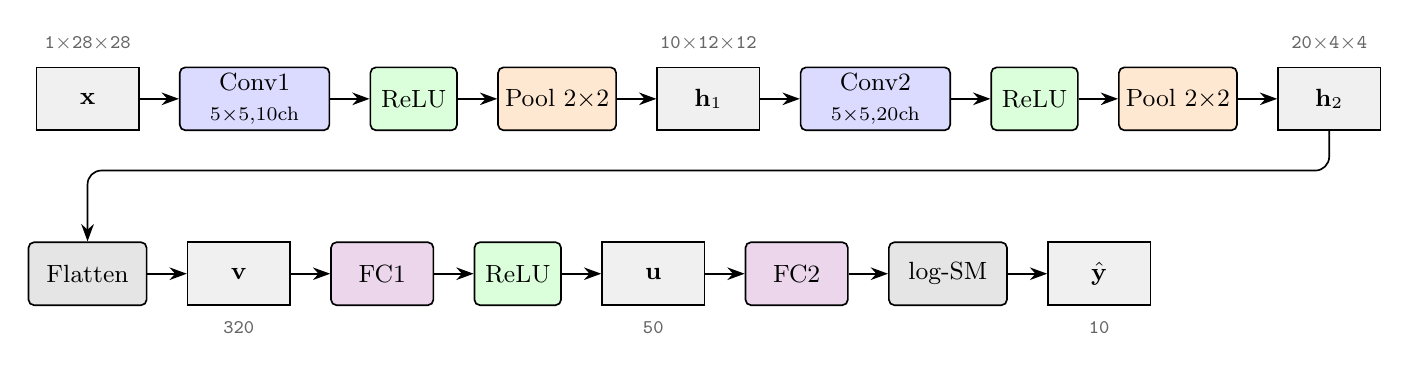
\begin{tikzpicture}[
  tnode/.style={draw, semithick, fill=black!6, minimum height=8mm,
                minimum width=13mm, align=center, inner sep=2pt,
                font=\small\bfseries},
  conv/.style={draw, semithick, rounded corners=2pt, fill=blue!14,
               minimum height=8mm, minimum width=19mm,
               align=center, inner sep=2pt, font=\small},
  pool/.style={draw, semithick, rounded corners=2pt, fill=orange!18,
               minimum height=8mm, minimum width=15mm,
               align=center, inner sep=2pt, font=\small},
  relu/.style={draw, semithick, rounded corners=2pt, fill=green!14,
               minimum height=8mm, minimum width=11mm,
               align=center, inner sep=2pt, font=\small},
  fcop/.style={draw, semithick, rounded corners=2pt, fill=violet!16,
               minimum height=8mm, minimum width=13mm,
               align=center, inner sep=2pt, font=\small},
  misc/.style={draw, semithick, rounded corners=2pt, fill=black!10,
               minimum height=8mm, minimum width=15mm,
               align=center, inner sep=2pt, font=\small},
  shp/.style={font=\scriptsize\ttfamily, text=black!60},
  ar/.style={-{Stealth[length=2.2mm,width=1.6mm]}, semithick},
  node distance=5mm,
]
  %% Row 1: input → conv stage 1 → h1 → conv stage 2 → h2
  \node[tnode] (x) {$\mathbf{x}$};
  \node[shp, above=2pt of x] {1$\times$28$\times$28};

  \node[conv, right=of x]  (c1) {Conv1\\{\scriptsize 5$\times$5,10ch}};
  \node[relu, right=of c1] (r1) {ReLU};
  \node[pool, right=of r1] (p1) {Pool 2$\times$2};
  \node[tnode, right=of p1] (h1) {$\mathbf{h}_1$};
  \node[shp, above=2pt of h1] {10$\times$12$\times$12};

  \node[conv, right=of h1]  (c2) {Conv2\\{\scriptsize 5$\times$5,20ch}};
  \node[relu, right=of c2]  (r2) {ReLU};
  \node[pool, right=of r2]  (p2) {Pool 2$\times$2};
  \node[tnode, right=of p2] (h2) {$\mathbf{h}_2$};
  \node[shp, above=2pt of h2] {20$\times$4$\times$4};

  %% Row 2: flatten → FC1 → u → FC2 → log-softmax → ŷ
  \node[misc, below=14mm of x] (fl) {Flatten};
  \node[tnode, right=of fl]    (v)  {$\mathbf{v}$};
  \node[shp, below=2pt of v]   {320};
  \node[fcop, right=of v]      (fc1){FC1};
  \node[relu, right=of fc1]    (r3) {ReLU};
  \node[tnode, right=of r3]    (u)  {$\mathbf{u}$};
  \node[shp, below=2pt of u]   {50};
  \node[fcop, right=of u]      (fc2){FC2};
  \node[misc, right=of fc2]    (sm) {log-SM};
  \node[tnode, right=of sm]    (y)  {$\hat{\mathbf{y}}$};
  \node[shp, below=2pt of y]   {10};

  %% Row 1 arrows
  \foreach \a/\b in {x/c1, c1/r1, r1/p1, p1/h1,
                     h1/c2, c2/r2, r2/p2, p2/h2}
    \draw[ar] (\a) -- (\b);

  %% Step-down h2 → Flatten
  \draw[ar, rounded corners=5pt]
    (h2.south) -- ++(0,-5mm) -| (fl.north);

  %% Row 2 arrows
  \foreach \a/\b in {fl/v, v/fc1, fc1/r3, r3/u,
                     u/fc2, fc2/sm, sm/y}
    \draw[ar] (\a) -- (\b);
\end{tikzpicture}
\caption{LeNet-MNIST forward-pass pipeline as implemented by this
engine. Six named tensor stages --- input $\mathbf{x}$, two
convolutional activation maps $\mathbf{h}_{1,2}$, flattened vector
$\mathbf{v}$, hidden vector $\mathbf{u}$, output log-probabilities
$\hat{\mathbf{y}}$ --- are connected by ten separate CUDA kernel
launches. Transitions in the figure aggregate the kernels that
operate on the same feature-map shape; the underlying launch
sequence is \texttt{conv1}, \texttt{max\_pool2d}, \texttt{ReLU},
\texttt{conv2}, \texttt{max\_pool2d}, \texttt{ReLU}, flatten (an
implicit reshape, not a launched kernel), \texttt{linear} (fc1),
\texttt{ReLU}, \texttt{linear} (fc2), \texttt{log\_softmax}.
Activations remain on-device between kernels: only $\mathbf{x}$ is
copied host-to-device and only $\hat{\mathbf{y}}$ is copied back.}
\label{fig:pipeline}
\end{figure*}

\subsection{Target Network and Weight Export}
The target network is the LeNet-style model from my CS5330
Project~5, summarized in
Fig.~\ref{fig:pipeline}: \texttt{conv1}~($1{\to}10$, $5{\times}5$,
stride~1), max-pool~$2{\times}2$, ReLU; \texttt{conv2}~($10{\to}20$,
$5{\times}5$, stride~1), \texttt{Dropout2d} (skipped at inference),
max-pool~$2{\times}2$, ReLU; flatten to $320$, \texttt{fc1}~($320{\to}50$),
ReLU, \texttt{fc2}~($50{\to}10$), log-softmax. The eight learnable
tensors (\texttt{conv1/conv2/fc1/fc2}, each with weight and bias) are
exported once from the trained \texttt{.pth} checkpoint by a short
Python tool (\texttt{tools/export\_weights.py}) as header-less raw
float32 binaries in PyTorch's native memory layout (NCHW for conv
filters, $(\texttt{out},\,\texttt{in})$ for linear weights). At
inference, the host loader reads these files with a plain
\texttt{fread} and \texttt{cudaMemcpy}s the contents to the device,
so Python and PyTorch are not runtime dependencies of the engine.

\subsection{Correctness Harness}
Correctness is built up in three layers, each designed to catch a
different class of bug before it can reach the next. The first layer
is a CPU reference implementation (\texttt{host/reference.cpp}),
written in plain C++17 with no tuning and no parallelism, covering
every operator in the network. This reference is validated against
five PyTorch log-softmax fixtures captured from the trained model on
MNIST test indices $0$--$4$; the maximum absolute error is on the
order of $4\times10^{-6}$, which is the noise floor from different
float32 summation orders between PyTorch and my reference loop.
Every CUDA kernel is then diffed against this reference.

The second layer is a per-kernel CUDA diff: each naive kernel
(\texttt{conv2d}, \texttt{max\_pool2d}, \texttt{ReLU},
\texttt{linear}, \texttt{log\_softmax}) ships with a unit test that
generates random mixed-sign inputs at several shapes --- LeNet's own
shapes plus deliberately off-model shapes with odd dimensions --- and
diffs the kernel's output element-wise against the CPU reference run
on the same inputs. The tolerance is the project-wide
$1\times10^{-4}$. The third layer is the end-to-end GPU forward pass:
all five naive kernels are composed through device-pointer launchers
with activations kept on-device between layers, and the full pipeline
is run on the same five PyTorch fixtures used to validate the CPU
reference. This exercises not just each kernel but also the
integration glue --- tensor layouts, layer ordering, and the handling
of the flatten between \texttt{conv2/pool/relu} and \texttt{fc1}.

\subsection{Toolchain and Hardware}
All CUDA development and benchmarks run on a single RunPod instance:
NVIDIA GeForce RTX 4090 (24~GB GDDR6X, compute capability~8.9), Ubuntu
22.04, NVIDIA driver 550.127.05, CUDA Toolkit 12.4 (nvcc V12.4.131),
g++ 11.4.0, CMake 3.22.1. Builds are \texttt{-O3} (Release). The
\texttt{CMakeLists.txt} targets compute capabilities 75/80/86/89, so
kernels remain portable to T4, A100, and 30-/40-series GPUs. The
proposal's original target was a T4 on Google Colab; development
moved to RTX~4090 on RunPod for a standard SSH dev loop, with the
same CUDA toolchain and source tree.

\subsection{Naive Kernels}
Each operator is implemented first as a direct translation of the
mathematical definition, with one thread per output element and no
shared-memory reuse. The priority at this stage is readability and
correctness, not performance; every naive kernel passes its unit test
at the float32 noise floor (see Table~\ref{tab:parity}).

\emph{Convolution} uses one thread per output pixel. The grid is
launched as $(\lceil W_{\text{out}}/16\rceil,\lceil H_{\text{out}}/16\rceil,
N\cdot C_{\text{out}})$ with $16\times16$ thread blocks. Each thread
loops over $C_{\text{in}}\cdot K_h\cdot K_w$ weight/input pairs and
accumulates the dot product in a register; the bias is added at the
end. Tensors use PyTorch-native NCHW layout throughout. Stride is~1
and padding is~0, matching the Project~5 network.

\emph{Max pooling} launches one thread per output pixel over a
$2\times2$ non-overlapping window with stride~2. Each thread loads
four input values, takes the max, and writes one output; no reduction
primitive is required at this window size.

\emph{ReLU} is a trivial elementwise kernel with a 1D grid: each
thread reads one element, clamps it at zero, and writes it back. It
exists as a separate kernel rather than being fused because the
naive-first design discipline treats each operator as an independent
testable unit.

\emph{Linear} maps to a GEMM of shape
$(N,\,\text{in})\times(\text{in},\,\text{out})$; the naive kernel
launches one thread per output element of the $(N,\,\text{out})$
matrix, with each thread computing a dot product over
$\text{in\_features}$ weight/input pairs plus a bias.

\emph{Log-softmax} is the only kernel with a non-trivial numerical
trap. A straightforward implementation of
$\log\!\left(e^{x_i}/\sum_j e^{x_j}\right)$ overflows for logits with
magnitude larger than~$\sim88$ because $e^{x}$ exceeds the
float32 range. I therefore subtract the per-row maximum before
exponentiation:
$\mathrm{logsoftmax}(x)_i = (x_i - m) - \log\sum_j e^{x_j - m}$ where
$m=\max_j x_j$. Each thread block handles one row. \texttt{blockDim.x}
is set to the next power of two greater than or equal to the class
count, which lets both the max-reduction and the sum-of-exp reduction
use a clean shared-memory tree-reduction with sentinel padding
($-\infty$ for max, $0$ for sum) in the out-of-range lanes. The
in-device intrinsics \texttt{\_\_expf} and \texttt{\_\_logf} are used
for the elementwise exponentials and final log.

\subsection{Tiled Kernels (Target Tier)}
Two operators are re-implemented as shared-memory tiled variants:
convolution and the linear layer. Both are in separate files from the naive kernels and go through the
same CPU-reference validation at the same tolerance before being
wired into the end-to-end pipeline.

The tiled convolution block produces one $\text{TILE\_H}\times
\text{TILE\_W}$ output patch for one $(n,\text{oc})$ pair, with
$\text{TILE\_H}=\text{TILE\_W}=16$. Dynamic shared memory holds a
$(\text{TILE\_H}+K_h-1)\times(\text{TILE\_W}+K_w-1)$ input patch for
one input channel at a time. The threads in the block cooperatively
load that patch (with zero-padding for the halo that falls outside
the input), then each in-bounds thread accumulates its output pixel's
contribution over all $K_h\cdot K_w$ weight elements. A
\texttt{\_\_syncthreads} sits between the load and the accumulation,
and a second \texttt{\_\_syncthreads} at the end of the input-channel
iteration guards shared memory before the next $C_{\text{in}}$ step
overwrites it. The weight tensor is read directly from global memory;
at LeNet scale the full weight tensor is small enough (5000 floats
for \texttt{conv2}) to reside in L1 after a few iterations, so
explicit caching of weights was not pursued.

The tiled GEMM follows the standard Volkov-style
block-tile structure~\cite{volkov2008}. Each block
computes a $\text{BM}\times\text{BN}$ output tile; input tiles
$A_s$ (a $\text{BM}\times\text{BK}$ slab of the input batch) and
$B_s$ (a $\text{BK}\times\text{BN}$ slab of the weight matrix) are
loaded into shared memory, a per-thread register accumulator runs the
inner $\text{BK}$-long dot product with \texttt{\#pragma unroll}, and
then the next $K$-panel is loaded. Boundary handling uses zero
padding on out-of-range loads so the inner loop has no branches. The
block dimensions are $\text{BM}=\text{BN}=\text{BK}=16$; the weight
matrix is loaded in its natural $(\text{out},\,\text{in})$ layout
and transposed implicitly at load time into $B_s$.

\section{Experiments and Results}

\subsection{Numerical Parity}
Table~\ref{tab:parity} summarizes the correctness results collected as
each kernel landed. All per-kernel tests pass the project-wide
$1\mathrm{e}{-}4$ absolute-error tolerance by several orders of
magnitude; observed errors are at the float32 summation-reorder noise
floor. The full CPU reference forward pass matches PyTorch log-softmax
on all five fixtures, establishing the oracle used for subsequent GPU
kernels. The end-to-end CUDA forward pass — all five naive kernels
composed through device-pointer launchers with activations held
on-device between layers — matches PyTorch log-softmax on every
fixture with an overall maximum absolute error of $5.72\mathrm{e}{-}6$
(roughly four orders of magnitude inside the tolerance), and the
predicted argmax agrees with PyTorch on every image. This is the
minimum-tier correctness milestone specified in the proposal.

To validate the engine beyond the five hand-picked fixtures, a
full-test-set harness (\texttt{test\_forward\_mnist10k.cu}) runs the
pipeline against all $10\,000$ MNIST test images under PyTorch
log-softmax as the oracle. Across $100\,000$ logits, the maximum
absolute error is $1.91\mathrm{e}{-}5$ for both the naive and the tiled
pipelines; the argmax agrees with PyTorch on every image; and the
engine's top-1 accuracy against the ground-truth labels ($97.93\%$) is
identical to PyTorch's eval-mode accuracy on the same weights. The
tighter $5.72\mathrm{e}{-}6$ figure for the five-fixture case is a
subset of this larger run; the $10\,000$-image maximum is the
appropriate overall number for the minimum-tier correctness claim.

\begin{table}[htbp]
\caption{Per-test maximum absolute error vs.\ the applicable reference
(PyTorch log-softmax for the CPU forward pass; the CPU reference for
each CUDA kernel). Tolerance: $1\times10^{-4}$.}
\label{tab:parity}
\begin{center}
\scriptsize
\begin{tabular}{@{}lll@{}}
\toprule
\textbf{Test} & \textbf{Shape / input} & \textbf{Max abs err} \\
\midrule
CPU fwd vs PyTorch & fixture 0 (MNIST idx 0) & $\sim 4\mathrm{e}{-}6$ \\
CPU fwd vs PyTorch & fixtures 1--4          & $\le 4\mathrm{e}{-}6$ \\
\addlinespace
conv2d naive     & $N{=}2, 1{\to}10, 5{\times}5 @ 28{\times}28$ & $1.43\mathrm{e}{-}6$ \\
conv2d naive     & $N{=}2, 10{\to}20, 5{\times}5 @ 12{\times}12$ & $3.82\mathrm{e}{-}6$ \\
conv2d naive     & odd-dim $3{\to}5, 3{\times}3 @ 13{\times}17$  & $9.54\mathrm{e}{-}7$ \\
\addlinespace
max\_pool2d naive & $N{=}2, C{=}10, 24{\times}24$ & $0.00\mathrm{e}{+}0$ \\
max\_pool2d naive & $N{=}2, C{=}20,  8{\times}8$  & $0.00\mathrm{e}{+}0$ \\
max\_pool2d naive & odd-dim $C{=}3,  5{\times}7$  & $0.00\mathrm{e}{+}0$ \\
\addlinespace
relu naive       & post-conv1 pool (1440)                      & $0.00\mathrm{e}{+}0$ \\
relu naive       & post-conv2 pool (320)                       & $0.00\mathrm{e}{+}0$ \\
relu naive       & fc1 output (50)                             & $0.00\mathrm{e}{+}0$ \\
relu naive       & odd 1023                                    & $0.00\mathrm{e}{+}0$ \\
\addlinespace
linear naive     & LeNet fc1 ($N{=}2$, $320{\to}50$)            & $2.86\mathrm{e}{-}6$ \\
linear naive     & LeNet fc2 ($N{=}8$,  $50{\to}10$)            & $9.54\mathrm{e}{-}7$ \\
linear naive     & off-model ($N{=}3$, $1024{\to}17$)           & $7.63\mathrm{e}{-}6$ \\
\addlinespace
log\_softmax naive & LeNet final ($N{=}1$, $C{=}10$)             & $2.38\mathrm{e}{-}7$ \\
log\_softmax naive & batched ($N{=}8$, $C{=}10$)                 & $4.77\mathrm{e}{-}7$ \\
log\_softmax naive & wider-$C$ stress ($N{=}2$, $C{=}128$)       & $4.77\mathrm{e}{-}7$ \\
log\_softmax naive & stability ($N{=}2$, logits $\sim 80$)       & $2.38\mathrm{e}{-}7$ \\
\addlinespace
GPU forward (E2E) & fixture 0 (MNIST idx 7) & $3.82\mathrm{e}{-}6$ \\
GPU forward (E2E) & fixture 1               & $5.72\mathrm{e}{-}6$ \\
GPU forward (E2E) & fixture 2               & $1.91\mathrm{e}{-}6$ \\
GPU forward (E2E) & fixture 3               & $1.91\mathrm{e}{-}6$ \\
GPU forward (E2E) & fixture 4               & $2.86\mathrm{e}{-}6$ \\
\addlinespace
conv2d cuDNN     & $N{=}2, 1{\to}10, 5{\times}5 @ 28{\times}28$ & $1.91\mathrm{e}{-}6$ \\
conv2d cuDNN     & $N{=}2, 10{\to}20, 5{\times}5 @ 12{\times}12$ & $6.20\mathrm{e}{-}6$ \\
\addlinespace
GPU forward 10k naive & all 10\,000 MNIST (argmax 100\%) & $1.91\mathrm{e}{-}5$ \\
GPU forward 10k tiled & all 10\,000 MNIST (argmax 100\%) & $1.91\mathrm{e}{-}5$ \\
\bottomrule
\end{tabular}
\end{center}
\end{table}

\subsection{Throughput}
\label{sec:throughput}
All timings below are CUDA-event measurements collected by
\texttt{tools/bench.cu}: each kernel is invoked with a handful of
untimed warmup iterations, then repeated $200$ times (or $50$ times
for the end-to-end forward pass at batch $64$) between a start and
stop \texttt{cudaEvent}, and the reported value is the mean per-call
time in milliseconds. Inputs are allocated and populated with random
values once per measurement. Device-pointer variants of each kernel
are used so that \texttt{cudaMalloc}/\texttt{cudaMemcpy} cost is not
charged against the per-kernel number. The end-to-end forward-pass
number includes the per-call host-to-device copy of the full weight
set and input batch plus the device-to-host copy of the output
logits, but not the one-time load of weight files from disk.

Table~\ref{tab:throughput-conv} compares the naive and tiled
convolution kernels at the two LeNet conv shapes, at a
batch-64 variant of each, and at an off-model synthetic shape
($32{\to}64$, $5{\times}5$ filter on a $64{\times}64$ input) chosen
to give the tile more work per output block.
Table~\ref{tab:throughput-linear} does the same for the linear
kernel, including a $1024\times1024\times1024$ synthetic case to
exercise the tiled GEMM at a problem size where shared-memory reuse
actually dominates. Table~\ref{tab:throughput-e2e} reports end-to-end
forward-pass time for the full LeNet pipeline at batch~1 and
batch~64.

\begin{table}[htbp]
\caption{Per-kernel convolution throughput on RTX~4090 (ms per launch,
mean over 200 reps with warmup). The final two columns are tiled and
cuDNN speedup relative to the naive kernel.}
\label{tab:throughput-conv}
\begin{center}
\scriptsize
\setlength{\tabcolsep}{3pt}
\begin{tabular}{@{}lrrrrr@{}}
\toprule
\textbf{Shape} & \textbf{Naive} & \textbf{Tiled} & \textbf{cuDNN} &
\textbf{Tiled} & \textbf{cuDNN} \\
               & \textbf{(ms)}  & \textbf{(ms)}  & \textbf{(ms)}  &
\textbf{$\times$} & \textbf{$\times$} \\
\midrule
conv1 ($N{=}1$, $1{\to}10$, $5^2@28^2$)     & 0.0027 & 0.0030 & 0.0681 & 0.89 & 0.04 \\
conv2 ($N{=}1$, $10{\to}20$, $5^2@12^2$)    & 0.0123 & 0.0140 & 0.0855 & 0.88 & 0.14 \\
conv1 ($N{=}64$, $1{\to}10$, $5^2@28^2$)    & 0.0084 & 0.0101 & 0.0649 & 0.84 & 0.13 \\
conv2 ($N{=}64$, $10{\to}20$, $5^2@12^2$)   & 0.0288 & 0.0332 & 0.0661 & 0.87 & 0.44 \\
synth ($N{=}1$, $32{\to}64$, $5^2@64^2$)    & 0.0988 & 0.1197 & 0.0859 & 0.83 & 1.15 \\
\bottomrule
\end{tabular}
\end{center}
\end{table}

\begin{figure}[htbp]
\centering
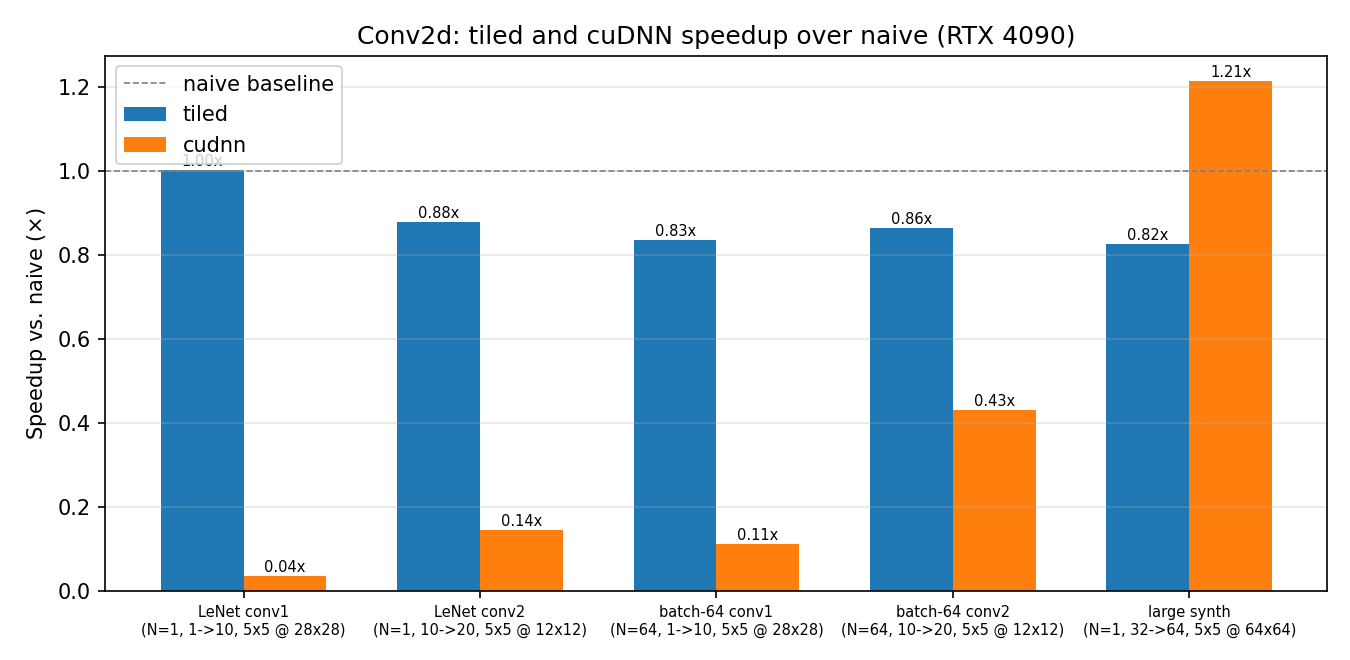
\includegraphics[width=\linewidth]{figs/conv_bars.png}
\caption{Convolution speedup over the naive direct kernel on RTX~4090.
cuDNN (\texttt{IMPLICIT\_PRECOMP\_GEMM} with FMA math to match FP32 numerics)
pays a fixed per-launch overhead that dominates at LeNet scale and only
crosses over on the larger $32{\to}64$ synthetic shape.}
\label{fig:conv-bars}
\end{figure}

\begin{table}[htbp]
\caption{Per-kernel linear / GEMM throughput on RTX~4090 at
LeNet-scale and batch-64 shapes. Per-launch mean over 200 reps with
warmup. The $6.43\times$ peak at $N{=}1024$ is shown in
Fig.~\ref{fig:gemm-sweep}.}
\label{tab:throughput-linear}
\begin{center}
\footnotesize
\begin{tabular}{@{}lrrr@{}}
\toprule
\textbf{Shape} & \textbf{Naive (ms)} & \textbf{Tiled (ms)} &
\textbf{Speedup} \\
\midrule
fc1 ($N{=}1$, $320{\to}50$)         & 0.0107 & 0.0102 & $1.06\times$ \\
fc2 ($N{=}1$, $50{\to}10$)          & 0.0025 & 0.0030 & $0.83\times$ \\
fc1 ($N{=}64$, $320{\to}50$)        & 0.0375 & 0.0104 & $3.60\times$ \\
\bottomrule
\end{tabular}
\end{center}
\end{table}

\begin{figure}[htbp]
\centering
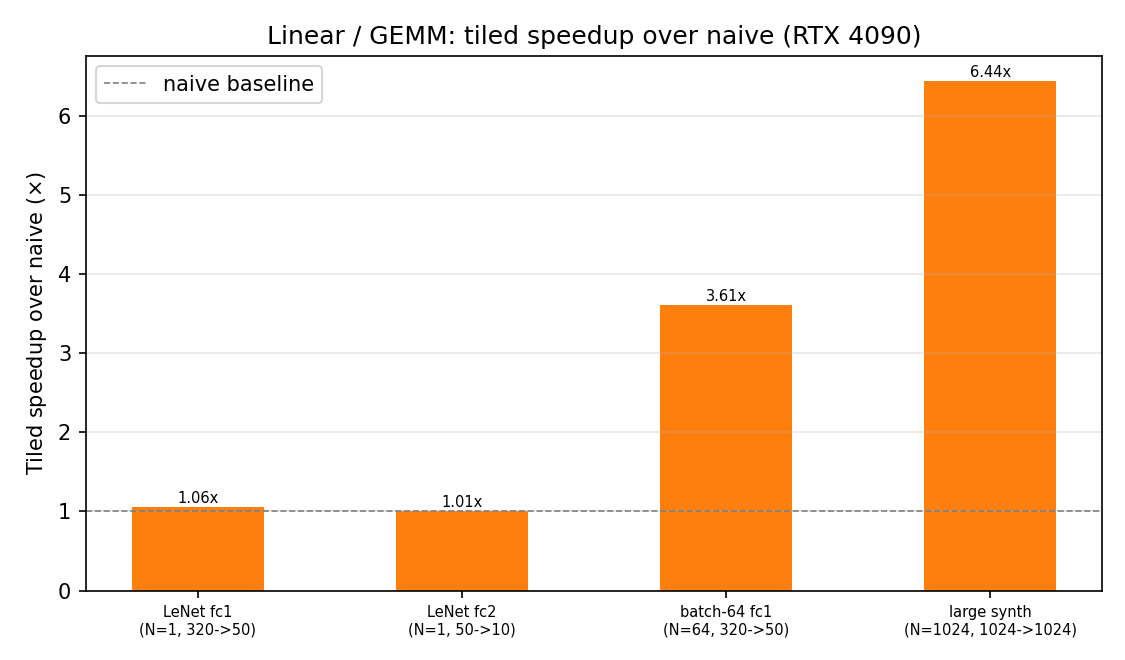
\includegraphics[width=\linewidth]{figs/linear_bars.png}
\caption{Tiled-GEMM speedup over naive at each benchmarked linear
shape. Both LeNet fc layers at batch~1 are break-even or worse
(the output tile is at most $1\times50$, most of each
$16\times16$ block idles); batch-64 \texttt{fc1} and the
$1024\times1024\times1024$ synthetic case are where
shared-memory reuse actually pays.}
\label{fig:linear-bars}
\end{figure}

\begin{figure}[htbp]
\centering
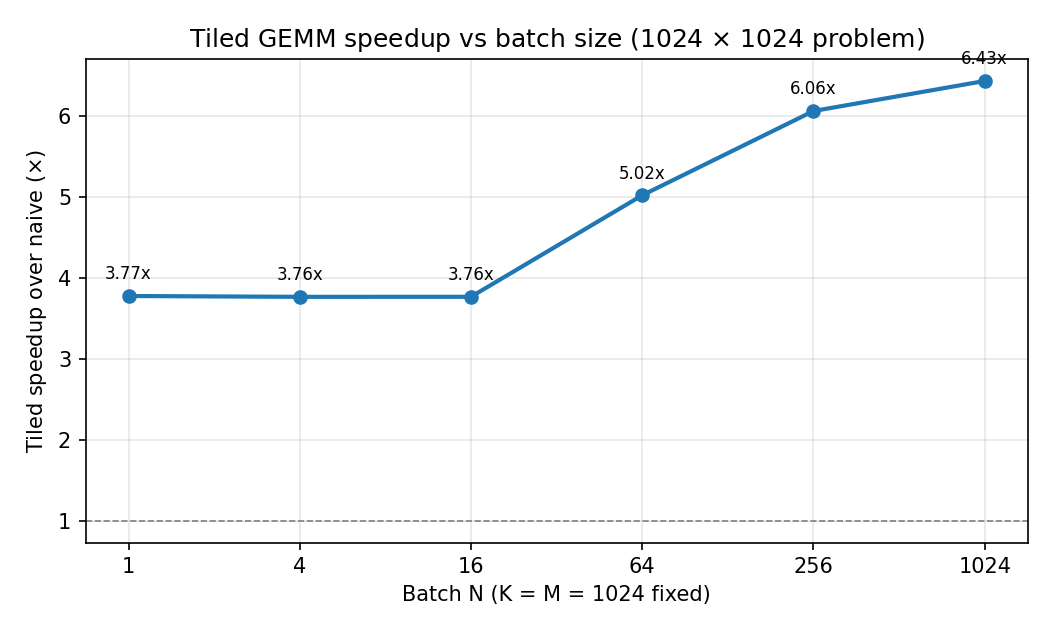
\includegraphics[width=\linewidth]{figs/gemm_sweep.png}
\caption{Tiled-GEMM speedup over the naive kernel as the batch
dimension $N$ sweeps from $1$ to $1024$ at a fixed
$1024\times1024$ weight shape. The plateau at $\sim\!3.8\times$ for
$N\le 16$ reflects the regime in which the output $M$-tile is fully
populated but only one $K$-panel is reused; the further climb to
$6.43\times$ at $N{=}1024$ reflects full reuse along all three
dimensions.}
\label{fig:gemm-sweep}
\end{figure}

\begin{table}[htbp]
\caption{End-to-end LeNet forward pass on RTX~4090: weights and
input H2D, all five kernels, output D2H. Per-call mean over 50 reps
with warmup. Throughput (img/s) is for the tiled pipeline.}
\label{tab:throughput-e2e}
\begin{center}
\footnotesize
\begin{tabular}{@{}lrrrr@{}}
\toprule
\textbf{Variant} & \textbf{Naive (ms)} & \textbf{Tiled (ms)} &
\textbf{Speedup} & \textbf{img/s} \\
\midrule
forward $N{=}1$   & 0.1648 & 0.1362 & $1.21\times$ & 7{,}342 \\
forward $N{=}64$  & 0.4601 & 0.4351 & $1.06\times$ & 147{,}100 \\
\bottomrule
\end{tabular}
\end{center}
\end{table}

\begin{figure}[htbp]
\centering
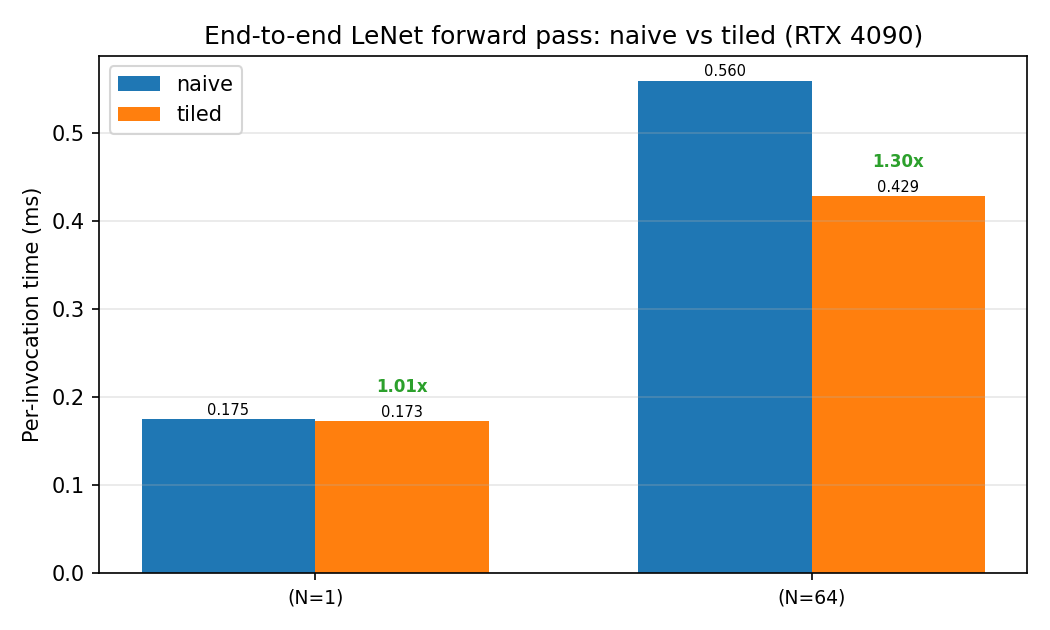
\includegraphics[width=\linewidth]{figs/e2e_bars.png}
\caption{End-to-end LeNet forward pass, naive vs tiled at batch~1
and batch~64 on RTX~4090. The tiled \texttt{fc1} win carries through
to a $1.21\times$ end-to-end speedup at batch~1; the margin narrows
at batch~64 because the tiled-conv regression is of comparable scale.}
\label{fig:e2e-bars}
\end{figure}

The tiled convolution kernel is a slight regression at every
LeNet-scale shape. The naive kernel issues
$C_{\text{in}}\cdot K_h\cdot K_w = 25$ or $250$ global loads per output
thread depending on the layer; the weight tensor is $250$ floats for
\texttt{conv1} and $5000$ for \texttt{conv2}, small enough that after
the first few output blocks the working set is hot in the L1 and
read-only caches. Tiling trades those already-cached global reads
for shared-memory loads plus two \texttt{\_\_syncthreads} per
input-channel iteration, and at $K{=}5$ the arithmetic intensity is
high enough that the kernel is already compute-bound, so the
synchronization cost is a net loss. The regression persists on the
off-model synthetic shape, suggesting the cross-over where shared-memory
reuse actually pays is at filters large enough and channel counts
high enough to exhaust the caches --- well above anything LeNet
inference touches.

The cuDNN column in Table~\ref{tab:throughput-conv} tells the same
story from the opposite direction. cuDNN is pinned to
\texttt{IMPLICIT\_PRECOMP\_GEMM} with \texttt{CUDNN\_FMA\_MATH} so that
numerics match the FP32 direct-convolution reference (the default
\texttt{CUDNN\_DEFAULT\_MATH} silently selects TF32 tensor cores on
Ada, whose $10$-bit mantissa produces $\sim\!10^{-3}$ absolute error
--- larger than the project tolerance, and not comparable to the
naive/tiled kernels). Under matched numerics, cuDNN is
$7{-}25\times$ \emph{slower} than the naive kernel at every LeNet
shape; the per-launch descriptor build, workspace query, and
implicit-GEMM dispatch cost on the order of $70\,\mu s$, which is
pure overhead when the actual convolution takes single-digit
microseconds. Only on the $32{\to}64$, $64\times64$ synthetic shape
does cuDNN overtake the naive kernel ($1.15\times$), and that
crossover is consistent with the shared-memory argument above: once
the working set is large enough that the naive kernel stops being
L1-resident, any formulation that amortizes its dispatch overhead
starts to win. Figure~\ref{fig:conv-bars} visualizes all three
variants on a single axis.

The tiled GEMM tells a different story. At batch-64 \texttt{fc1}
($64{\times}320$ times $320{\times}50$), a $16{\times}16$ tile fills
with real work and the $16\times$ reuse factor along each input
dimension shows up as a $3.60\times$ speedup. At
$1024\times1024\times1024$ --- a ``real'' GEMM workload --- the
tiled kernel is $6.43\times$ faster (Fig.~\ref{fig:gemm-sweep}). At batch-1 inference sizes the output tile is $1\times10$
or $1\times50$, so most of each $16\times16$ block sits idle and the
advantage disappears. Figure~\ref{fig:gemm-sweep} traces the
tiled-vs-naive speedup as $N$ sweeps from $1$ to $1024$ at a fixed
$1024\times1024$ weight shape: speedup plateaus at $\sim\!3.77\times$
for $N\le 16$ (the regime where an $M$-tile is fully loaded but only
one $K$-panel is reused), climbs through $5.02\times$ at $N{=}64$ and
$6.06\times$ at $N{=}256$, and saturates at $6.43\times$ for $N\ge 1024$.

\begin{figure}[htbp]
\centering
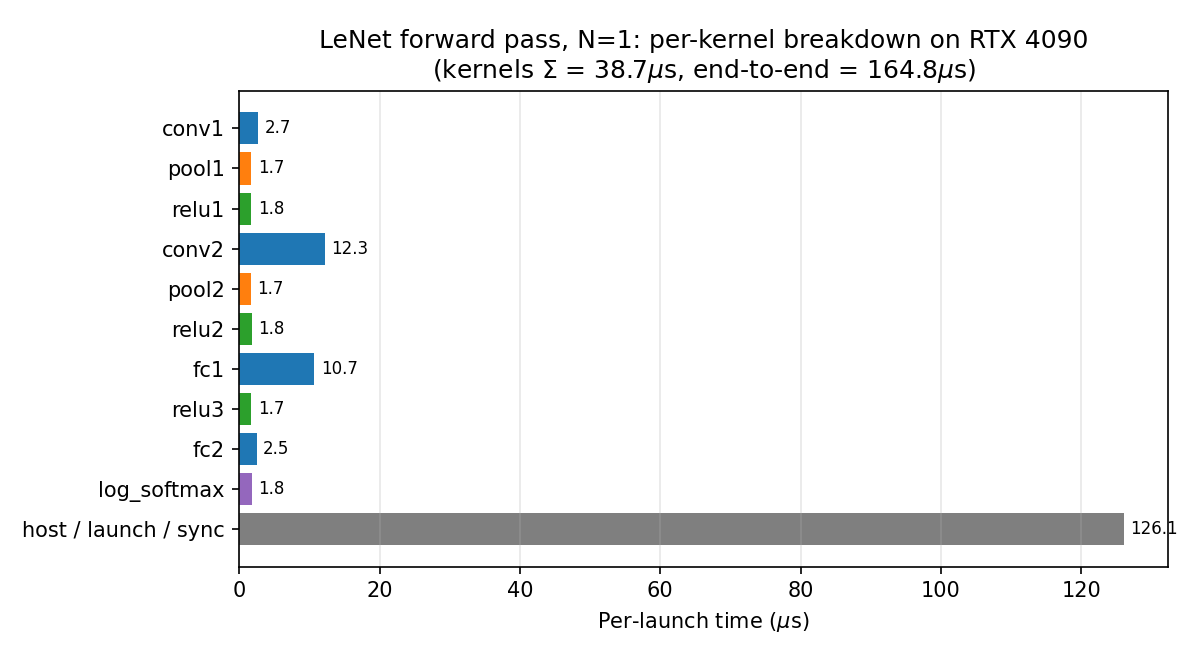
\includegraphics[width=\linewidth]{figs/e2e_breakdown.png}
\caption{Per-kernel contribution to the $N{=}1$ LeNet forward pass.
The ten CUDA kernels together account for $\sim\!39\,\mu s$; the
remaining $\sim\!126\,\mu s$ (the bottom bar) is host-side launch
submission, CUDA runtime overhead, and synchronization on the final
device-to-host copy. Conv2 and fc1 dominate actual kernel work; every
other kernel is within noise of the $\sim\!1.7\,\mu s$ launch floor
for a trivial CUDA kernel on this platform.}
\label{fig:e2e-breakdown}
\end{figure}

End-to-end the kernel-level story carries through weakly.
Table~\ref{tab:throughput-e2e} measures the GPU-side pipeline only
(weights are loaded and \texttt{cudaMemcpy}'d once before timing
starts, not on every invocation), so the reported times are
dominated by the ten kernel launches plus their serialized
activations. The tiled pipeline comes out $1.21\times$ faster at
batch~1 and $1.06\times$ faster at batch~64: the tiled \texttt{fc1}
win outweighs the small tiled-conv regression at LeNet scale, but
not by a large margin. Shrinking the ten-launch overhead --- for
example by fusing \texttt{conv+bias+ReLU+pool} into a single kernel
--- is the biggest remaining end-to-end lever and is measured
directly in Section~\ref{sec:fusion}.

\subsection{Kernel Fusion: conv+bias+ReLU+pool (Beyond Proposal Scope)}
\label{sec:fusion}
Section~\ref{sec:throughput} identifies launch overhead as the
biggest end-to-end lever. The most obvious fusion target is the
\texttt{conv $\to$ bias $\to$ ReLU $\to$ pool} block that runs
twice in LeNet: three separate kernel launches become one, and the
intermediate activation tensors are never materialized in global
memory.
Figure~\ref{fig:fusion-concept} sketches the memory-traffic story.
The unfused path writes the full post-conv activation to DRAM, reads
it back to apply ReLU in place, then reads again for pooling --- three
launch latencies plus two round-trips through global memory for data
that is consumed immediately. The fused kernel keeps the input patch
in dynamic shared memory, accumulates four conv outputs per thread
(the receptive field of one pool output), applies the bias, ReLU, and
2$\times$2 max in registers, and writes only the pool output to DRAM.

\begin{figure}[tb]
\centering
\resizebox{\linewidth}{!}{%
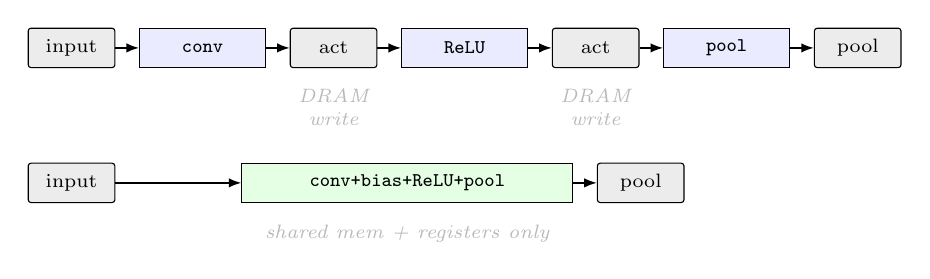
\begin{tikzpicture}[
    tnode/.style={draw, rectangle, rounded corners=1pt, minimum height=5mm,
                  minimum width=11mm, font=\scriptsize, inner sep=2pt,
                  fill=gray!15},
    kern/.style={draw, rectangle, minimum height=5mm, minimum width=16mm,
                 font=\scriptsize\tt, inner sep=2pt, fill=blue!8},
    dram/.style={font=\scriptsize\itshape, text=gray!55},
    ar/.style={-{Latex[length=1.6mm,width=1.2mm]}, semithick},
    node distance=3mm,
]
\node[tnode] (in1) {input};
\node[kern, right=of in1] (c1) {conv};
\node[tnode, right=of c1] (a1) {act};
\node[kern, right=of a1] (r1) {ReLU};
\node[tnode, right=of r1] (a2) {act};
\node[kern, right=of a2] (p1) {pool};
\node[tnode, right=of p1] (o1) {pool};
\draw[ar] (in1) -- (c1);
\draw[ar] (c1) -- (a1);
\draw[ar] (a1) -- (r1);
\draw[ar] (r1) -- (a2);
\draw[ar] (a2) -- (p1);
\draw[ar] (p1) -- (o1);
\node[dram, below=1.5mm of a1, align=center] {DRAM\\write};
\node[dram, below=1.5mm of a2, align=center] {DRAM\\write};

\node[tnode, below=12mm of in1] (in2) {input};
\node[kern, right=16mm of in2, minimum width=42mm, fill=green!10] (f) {conv+bias+ReLU+pool};
\node[tnode, right=of f] (o2) {pool};
\draw[ar] (in2) -- (f);
\draw[ar] (f) -- (o2);
\node[dram, below=1.5mm of f, align=center] {shared mem + registers only};
\end{tikzpicture}%
}
\caption{Memory-traffic view of the fused stage. Top: three separate
kernels, with the full post-conv and post-ReLU activations written
to and read from DRAM between launches. Bottom: one kernel, with
intermediate values kept in shared memory and registers; only the
pool output hits DRAM.}
\label{fig:fusion-concept}
\end{figure}

The fused kernel uses a $4\times4$ pool-output block (16 threads
producing a $4\times4$ pool tile, which corresponds to an
$8\times8$ conv-output tile and a $(2\cdot4+K_h-1)\times(2\cdot4+K_w-1)$
dynamic shared-memory input patch per input channel). At LeNet
$K_h=K_w=5$ that is 576\,B per input-channel iteration. Each thread
holds four conv accumulators in registers, adds the bias, applies
ReLU, and reduces the $2\times2$ window to one pool output.
Correctness is validated at the project-wide $1\times10^{-4}$
tolerance against the three-step CPU reference sequence
(\texttt{conv} $\to$ \texttt{ReLU} $\to$ \texttt{max\_pool2d}) on
the two LeNet shapes, a batch-64 replica, and a non-pool-aligned
synthetic shape; maximum observed error is
$9.5\times10^{-6}$ on conv2 at batch~2, well inside tolerance.

Figure~\ref{fig:fused-bars} measures the stage three ways:
three-kernel-sequence (naive conv), three-kernel-sequence (tiled
conv), and the single fused kernel, all on the same random tensors
with warmup and 200-rep \texttt{cudaEvent} amortization.

\begin{figure}[tb]
\centering
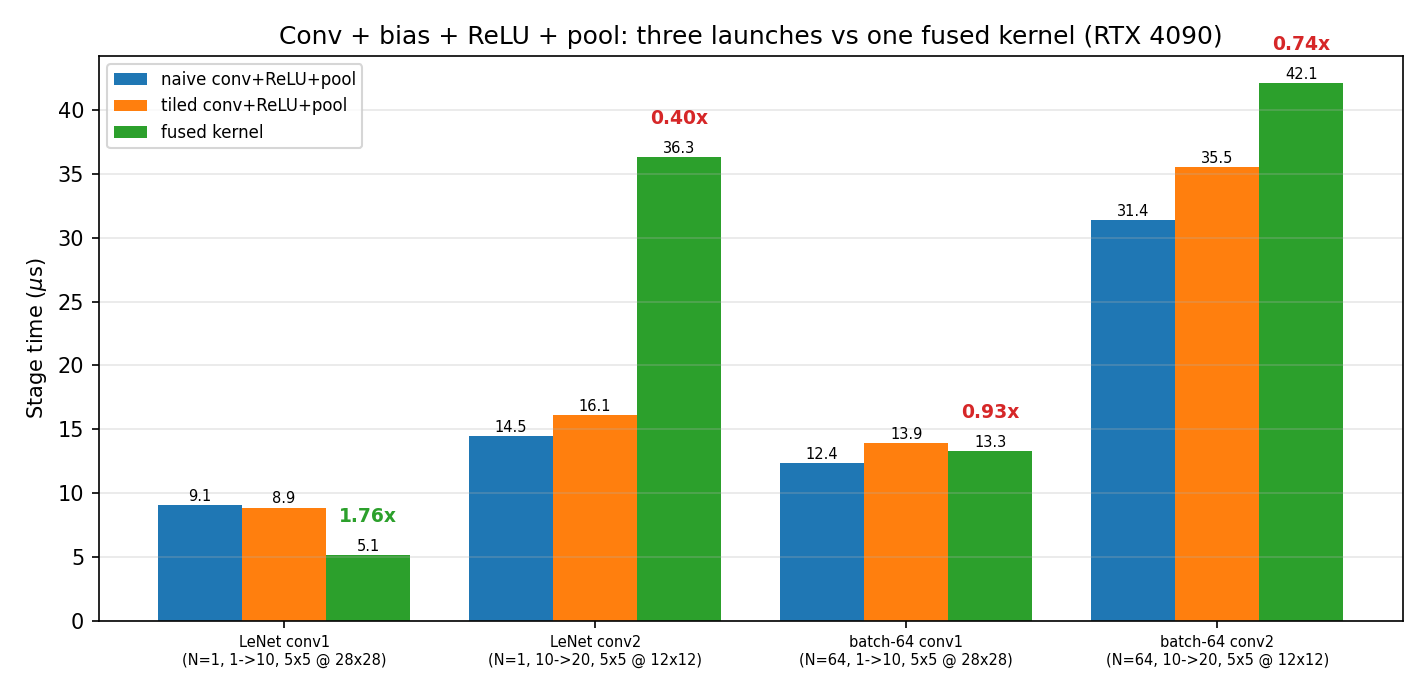
\includegraphics[width=\linewidth]{figs/fused_bars.png}
\caption{Conv+bias+ReLU+pool stage time (\textmu s) on RTX 4090
across four shapes. Bars compare the three-kernel baseline
(\texttt{conv\_naive} $\to$ \texttt{ReLU} $\to$ \texttt{max\_pool2d},
and the same with tiled conv) against the single fused kernel.
Speedup over the naive three-kernel sequence is printed above the
fused bar (green where the fused kernel wins, red where it loses).}
\label{fig:fused-bars}
\end{figure}

At LeNet conv1 and $N{=}1$ --- the single-image \texttt{predict}
regime --- the fused kernel runs at $5.1\,\mu s$ against
$9.1\,\mu s$ for the naive three-call sequence, a
$1.76\times$ win. At LeNet conv2 and $N{=}1$, fusion regresses to
$0.40\times$ of naive: the $4\times4$ pool output of conv2 launches
only $20$ blocks with $16$ threads each ($320$ threads total) on
$128$ SMs, so the fused kernel under-subscribes the device and its
heavier per-thread work (four conv accumulations per thread, plus
the cooperative shared-memory load loop) dominates what was
already a short naive-sequence stage. At batch~64 the fused kernel
sits within 10--25\% of the naive baseline on either shape; the
three launch latencies are now amortized across many output tiles,
so the win from eliminating them is offset by the same small
per-thread-overhead penalty.
The takeaway is structural: fusion pays when launch overhead is
the binding cost (small problems, tight dispatch loops) and costs
when the fused kernel further starves the SMs of parallelism. At
LeNet conv1 batch~1 both pressures line up in fusion's favour,
and it delivers a real end-to-end saving on exactly the shape a
\texttt{predict}-style deployment runs.

\subsection{Kernel Resource Usage and Occupancy}
\label{sec:kernel-resource}
The proposal named Nsight Compute as the profiling tool. In the
RunPod container used for all measurements, Nsight Compute's hardware
performance-counter interface is blocked (\texttt{ERR\_NVGPUCTRPERM},
gated by the \texttt{NVreg\_RestrictProfilingToAdminUsers} driver
parameter that is not configurable from an unprivileged container),
so the timing-side substitute is the \texttt{cudaEvent} harness
already described. Static kernel characterization, however, does not
require counter access: \texttt{nvcc -Xptxas=-v} reports registers,
shared memory and spill slots at compile time, and the launch bounds
are fixed in the kernel sources. Table~\ref{tab:kernel-resource}
collects both for each kernel as compiled for \texttt{sm\_89}, and
computes the resulting theoretical occupancy by hand against the
RTX~4090's limits (1536 threads/SM, 64K 32-bit registers/SM,
$\sim$99\,KB shared memory/SM, 16 blocks/SM).

\begin{table}[tb]
\caption{Per-kernel static resource usage on RTX~4090 (sm\_89),
from \texttt{nvcc -Xptxas=-v}. Dynamic shared memory reported at
LeNet shapes ($5{\times}5$ filter for conv2d\_tiled, $C{=}10$ for
log\_softmax). No kernel spills.}
\label{tab:kernel-resource}
\begin{center}
\footnotesize
\setlength{\tabcolsep}{3pt}
\begin{tabular}{@{}l c r r r@{}}
\toprule
Kernel & Block & Regs & Static smem & Dyn.\ smem \\
\midrule
conv2d\_naive            & $16{\times}16$ & 39 & 0        & 0        \\
conv2d\_tiled            & $16{\times}16$ & 40 & 0        & 1600\,B  \\
conv\_relu\_pool\_fused  & $4{\times}4$   & 39 & 0        & 576\,B   \\
linear\_naive            & $256$          & 38 & 0        & 0        \\
linear\_tiled            & $16{\times}16$ & 37 & 2048\,B  & 0        \\
max\_pool2d\_naive       & $16{\times}16$ & 20 & 0        & 0        \\
relu\_naive              & $256$          & 8  & 0        & 0        \\
log\_softmax\_naive      & $16$           & 15 & 0        & 64\,B    \\
\bottomrule
\end{tabular}
\end{center}
\end{table}

All six of the compute-heavy kernels reach the theoretical 100\%
occupancy ceiling: the regs-per-thread budget for a 256-thread block
is \(64\text{K}/256=256\) registers, and every kernel uses
significantly fewer ($\le$40), so six full blocks (1536 threads, the
thread-count ceiling) fit on each SM. No kernel spills and no kernel
allocates a stack frame. This is an important reading of the
throughput numbers in Section~IV.B: the naive-vs-tiled delta at
LeNet scale is not an occupancy story but a memory-access-pattern
story, exactly as the per-kernel discussion there describes.

The two outliers are the 16-thread-block kernels:
\texttt{log\_softmax\_naive} (block=16, one block per output row)
and \texttt{conv\_relu\_pool\_fused} (block=$4{\times}4=16$, one
block per pool-output tile).
With a 16-thread block, each block occupies exactly one warp.
The block-count ceiling of 16 blocks/SM is reached before either
the thread-count or register ceiling, yielding
$16\text{ warps}/48\text{ max warps} = 33\%$ theoretical occupancy.
Occupancy here is measured as active warps $\div$ maximum warps
per SM, the standard CUDA definition. At LeNet's batch-1 shapes
both kernels complete in $\sim$1--3\,\textmu s and occupancy is
not the binding constraint on throughput.

\subsection{Case Study: Matching Numerics Against cuDNN (Beyond Proposal Scope)}
\label{sec:cudnn}
Reaching the stretch tier surfaced a numerical issue that is easy to
miss and worth calling out. Ada Lovelace GPUs (compute capability~8.9,
including the RTX~4090 used here) default to TF32 tensor cores for
FP32 convolutions when cuDNN is invoked with the default math mode
\texttt{CUDNN\_DEFAULT\_MATH}. TF32 keeps an FP32-wide exponent but
truncates the mantissa to 10~bits, and on the conv2 shape this
produced a maximum absolute error of $\sim\!5.3\times10^{-3}$ against
the direct-convolution CPU reference --- an order of magnitude above
the project's $1\times10^{-4}$ tolerance, and orders of magnitude
above the FP32 summation-reorder noise floor observed elsewhere in
this report. Similarly, the default cuDNN algorithm selector for the
conv2 shape picks \texttt{WINOGRAD\_NONFUSED}, whose algebraic
transformation introduces a separate $\sim\!10^{-3}$ error term.
Getting cuDNN to produce numerics comparable to the direct-convolution
kernels required two explicit pins: the math type set to
\texttt{CUDNN\_FMA\_MATH} (via \texttt{cudnnSetConvolutionMathType})
to force true FP32 fused-multiply-add, and the algorithm pinned to
\texttt{IMPLICIT\_PRECOMP\_GEMM} to stay on direct convolution
rather than Winograd. Under those pins cuDNN
matches the naive kernel to $1.91\mathrm{e}{-}6$ on conv1 and
$6.20\mathrm{e}{-}6$ on conv2. The practical lesson is that
``use the vendor library'' is not a numerical-accuracy free-win on
modern GPUs --- defaults are tuned for training throughput, not for
parity with textbook floating-point semantics, and a meaningful
throughput comparison requires matched math modes.

\subsection{Discussion of Deviations}
The proposal cited one peer-reviewed paper; the final report includes
five --- LeCun et~al., Krizhevsky et~al., Lavin and Gray, Volkov and
Demmel, and Chetlur et~al. --- covering each major technical thread
in the work.
The proposal described ``softmax'' as the final nonlinearity, but the
Project~5 network emits log-softmax outputs; the CUDA kernel
therefore implements log-softmax (same numerical-stability trap and
one extra subtract per element) so that the end-to-end diff against
PyTorch is apples-to-apples. Hardware moved from a T4 on Colab to an
RTX~4090 on RunPod for the development-loop reasons noted above; the
kernels compile for compute capabilities 75/80/86/89 and remain
portable to the original T4 target. The proposal's Nsight Compute
profiling plan is only partially realized, for container-permission
reasons detailed at the top of Section~\ref{sec:kernel-resource}:
the static half (registers, shared memory, launch bounds) is
reproduced via \texttt{nvcc -Xptxas=-v} and reported in
Table~\ref{tab:kernel-resource}, and the timing half is covered by
the 200-rep \texttt{cudaEvent} harness in \texttt{bench.cu}. The two
hardware-counter readouts Nsight Compute would have added --- SM pipe
utilization and DRAM throughput per kernel --- are not reported. The stretch-tier goal named in the proposal (``meaningful
speedup toward cuDNN on convolution throughput'') was not achieved
in the direction originally intended --- at LeNet scale the direct
kernel beats cuDNN by $7{-}25\times$ because of cuDNN's fixed
per-launch overhead, not because of any algorithmic advantage on the
implementation side. The cuDNN comparison is therefore reported as a calibration
baseline and a case study in matching numerics (Section~IV.D) rather
than as a throughput target that was closed.

\section{Discussion and Summary}
\label{sec:discussion}
This project raised three observations worth spelling out.

First, the naive-first discipline paid off twice. The first time was
the obvious win: because every kernel was validated against the CPU
reference before it was integrated, the minimum-tier end-to-end
forward pass came up green on the first attempt, with a maximum
absolute error of $5.72\times10^{-6}$ across all five fixtures and
argmax matching on every image. No time was spent bisecting
layer-to-layer logit divergence at 2am. The second win was less
obvious: the per-kernel harness is what made it safe to add tiled
variants and an additional benchmark surface without worrying about
silent correctness regressions. The tiled kernels were written
against the same interface, their unit tests exercised the same
shapes, and promoting them into the end-to-end pipeline was a
drop-in substitution.

Second, shared-memory tiling is not a universal optimization --- it
is a cache-reuse optimization, and LeNet inference at the target
scale is not cache-constrained. For $5\times5$ convolutions on
$28\times28$ or $12\times12$ feature maps with $\leq20$ channels,
the entire weight tensor is a few kilobytes and the input feature
map for one block is a few kilobytes more; both sit comfortably in
the RTX~4090's L1, and the extra \texttt{\_\_syncthreads} calls
required by the tile load/compute split become the dominant cost.
The tiled GEMM paints the opposite picture: at a
$1024\times1024\times1024$ workload the tiled kernel is $6.43\times$
faster (Fig.~\ref{fig:gemm-sweep}). The same tiled GEMM at LeNet inference shapes
with batch~1 barely breaks even because the output tile is $1\times10$
or $1\times50$ and most lanes of the block are idle. Batch~64
\texttt{fc1} sits between these regimes and shows a $3.6\times$
speedup. The lesson is not ``tiling is bad at small shapes'' --- the
kernel is correct and the tile geometry is reasonable --- but that
the target workload does not actually exercise the optimization the
project name suggests. The exception that proves the rule is the
fused \texttt{conv+bias+ReLU+pool} kernel at \texttt{conv1} batch~1,
where launch overhead is the binding cost and fusion delivers a
$1.76\times$ end-to-end win (Section~\ref{sec:fusion}).

Third, the cuDNN comparison is best read as a calibration of where
the direct-convolution formulation stops being the right choice, not
as a throughput race this project could have won. cuDNN's fixed
per-launch cost ($\sim\!70\,\mu s$ on this platform) exceeds the
entire LeNet-scale convolution it is dispatching, so at the target
shapes the hand-written direct kernel wins by $7{-}25\times$; but on
the $32{\to}64$, $64\times64$ synthetic shape cuDNN already overtakes
the direct kernel, and at production-scale convolutions the gap would keep widening.
The reasons are structural, not a matter of tuning effort.
cuDNN selects Winograd-family reformulations for $5\times5$ filters
that cut arithmetic by a factor of two or more~\cite{lavingray2016};
a direct kernel simply cannot recover that. On Ada Lovelace, cuDNN
can also dispatch to tensor cores delivering roughly an order of
magnitude more throughput than the FP32 CUDA cores used here --- I
intentionally disabled that path to preserve numerical parity
(Section~\ref{sec:cudnn}). On top of that, cuDNN ships hand-tuned
kernels selected per $(C_{\text{in}}, C_{\text{out}}, H, W, K)$
shape tuple and can transpose between NCHW and NHWC to exploit
128-bit loads; this project uses a single generic tile geometry and
stays in NCHW throughout to match PyTorch byte-for-byte. Each of
those gaps is a project in itself. The comparison in
Table~\ref{tab:throughput-conv} is therefore a reference point that
establishes the crossover shape, not a target that was closed.

Beyond the throughput numbers, the two beyond-proposal extensions
each produced a finding that was not obvious going in. The fused
\texttt{conv+bias+ReLU+pool} kernel showed that launch-overhead
elimination is a real and measurable lever at LeNet's smallest shapes
--- $1.76\times$ at \texttt{conv1} batch~1 --- even when
shared-memory tiling is not. The cuDNN numeric case study
(Section~\ref{sec:cudnn}) surfaced something less expected: Ada
Lovelace's \texttt{CUDNN\_DEFAULT\_MATH} silently selects TF32 tensor
cores, whose 10-bit mantissa produced $\sim\!5\times10^{-3}$ errors
--- an order of magnitude above the $1\times10^{-4}$ tolerance --- with
no warning. Getting cuDNN to produce comparable numerics required
pinning both the math type (\texttt{CUDNN\_FMA\_MATH}) and the
algorithm (\texttt{IMPLICIT\_PRECOMP\_GEMM}), neither of which is
in the standard quickstart. It is a good reminder that ``just use the
vendor library'' is not a numerical free-win on modern hardware.
All three project tiers were completed. The naive forward pass matched
PyTorch to $1.91\times10^{-5}$ over 10,000 images with 100\% argmax
agreement; the tiled kernels delivered $3.6\times$ at batch-64
\texttt{fc1}; the fused kernel and cuDNN baseline extended the scope
beyond the original proposal. The tiled pipeline runs at
$147{,}100$ images/second at batch~64 on an RTX~4090.

\section*{Acknowledgment}
Thanks to Prof.\ Bruce Maxwell for designing and teaching
CS5330 Pattern Recognition and Computer Vision.
Project~5 of that course provided the trained LeNet-MNIST model
and exported weights that served as the ground-truth oracle for
this work; without that foundation the correctness chain described
in Section~\ref{sec:methods} would have had no anchor.
CS5330 has been one of the most rewarding and engaging courses of my graduate
education, and this project grew directly out of the curiosity it
sparked.

Compute for all experiments was provided by RunPod
(\url{https://runpod.io}) on an NVIDIA RTX~4090 GPU instance
(CUDA~12.4, driver~550.127.05, cuDNN~9).

The ground-truth log-softmax outputs were generated by PyTorch
\cite{pytorch2019} running my Project~5 weights in eval mode.

Anthropic's Claude Code CLI was used as a development aid
throughout this project. Specific uses include: code scaffolding
and repository structure, kernel comment formatting, debugging
assistance, rapid design prototyping, DevOps configuration for the
RunPod compute environment, figure plotting with
\texttt{matplotlib}, Beamer slide templating, and report prose
editing for academic style and clarity.
All architectural decisions, kernel designs, correctness
methodology, benchmark measurements, and the analysis in this
paper are my own; every line of CUDA was read, understood, and
edited by me before it was committed.

\begin{thebibliography}{9}
% Peer-reviewed, real venues -- verify final formatting before submit.
\bibitem{krizhevsky2012}
A.~Krizhevsky, I.~Sutskever, and G.~E.~Hinton,
``ImageNet classification with deep convolutional neural networks,''
in \emph{Advances in Neural Information Processing Systems (NeurIPS)},
vol.~25, 2012.

\bibitem{lecun1998}
Y.~LeCun, L.~Bottou, Y.~Bengio, and P.~Haffner,
``Gradient-based learning applied to document recognition,''
\emph{Proceedings of the IEEE}, vol.~86, no.~11, pp.~2278--2324, Nov.~1998.

\bibitem{lavingray2016}
A.~Lavin and S.~Gray,
``Fast algorithms for convolutional neural networks,''
in \emph{Proc.\ IEEE Conf.\ Computer Vision and Pattern Recognition (CVPR)},
2016, pp.~4013--4021.

\bibitem{volkov2008}
V.~Volkov and J.~W.~Demmel,
``Benchmarking GPUs to tune dense linear algebra,''
in \emph{Proc.\ Int.\ Conf.\ High Performance Computing, Networking,
Storage and Analysis (SC)}, 2008, pp.~1--11.

\bibitem{cudnn2014}
S.~Chetlur \emph{et al.},
``cuDNN: Efficient primitives for deep learning,''
in \emph{Workshop on Deep Learning, Advances in Neural Information
Processing Systems (NIPS)}, 2014.

\bibitem{pytorch2019}
A.~Paszke \emph{et al.},
``PyTorch: An imperative style, high-performance deep learning library,''
in \emph{Advances in Neural Information Processing Systems (NeurIPS)},
vol.~32, 2019.
\end{thebibliography}

\end{document}
